% Options for packages loaded elsewhere
\PassOptionsToPackage{unicode}{hyperref}
\PassOptionsToPackage{hyphens}{url}
%
\documentclass[
]{article}
\usepackage{amsmath,amssymb}
\usepackage{lmodern}
\usepackage{ifxetex,ifluatex}
\ifnum 0\ifxetex 1\fi\ifluatex 1\fi=0 % if pdftex
  \usepackage[T1]{fontenc}
  \usepackage[utf8]{inputenc}
  \usepackage{textcomp} % provide euro and other symbols
\else % if luatex or xetex
  \usepackage{unicode-math}
  \defaultfontfeatures{Scale=MatchLowercase}
  \defaultfontfeatures[\rmfamily]{Ligatures=TeX,Scale=1}
\fi
% Use upquote if available, for straight quotes in verbatim environments
\IfFileExists{upquote.sty}{\usepackage{upquote}}{}
\IfFileExists{microtype.sty}{% use microtype if available
  \usepackage[]{microtype}
  \UseMicrotypeSet[protrusion]{basicmath} % disable protrusion for tt fonts
}{}
\makeatletter
\@ifundefined{KOMAClassName}{% if non-KOMA class
  \IfFileExists{parskip.sty}{%
    \usepackage{parskip}
  }{% else
    \setlength{\parindent}{0pt}
    \setlength{\parskip}{6pt plus 2pt minus 1pt}}
}{% if KOMA class
  \KOMAoptions{parskip=half}}
\makeatother
\usepackage{xcolor}
\IfFileExists{xurl.sty}{\usepackage{xurl}}{} % add URL line breaks if available
\IfFileExists{bookmark.sty}{\usepackage{bookmark}}{\usepackage{hyperref}}
\hypersetup{
  pdftitle={Lab 11: Structural Bioinformatics (Pt. 1)},
  pdfauthor={Taylor Darby},
  hidelinks,
  pdfcreator={LaTeX via pandoc}}
\urlstyle{same} % disable monospaced font for URLs
\usepackage[margin=1in]{geometry}
\usepackage{color}
\usepackage{fancyvrb}
\newcommand{\VerbBar}{|}
\newcommand{\VERB}{\Verb[commandchars=\\\{\}]}
\DefineVerbatimEnvironment{Highlighting}{Verbatim}{commandchars=\\\{\}}
% Add ',fontsize=\small' for more characters per line
\usepackage{framed}
\definecolor{shadecolor}{RGB}{248,248,248}
\newenvironment{Shaded}{\begin{snugshade}}{\end{snugshade}}
\newcommand{\AlertTok}[1]{\textcolor[rgb]{0.94,0.16,0.16}{#1}}
\newcommand{\AnnotationTok}[1]{\textcolor[rgb]{0.56,0.35,0.01}{\textbf{\textit{#1}}}}
\newcommand{\AttributeTok}[1]{\textcolor[rgb]{0.77,0.63,0.00}{#1}}
\newcommand{\BaseNTok}[1]{\textcolor[rgb]{0.00,0.00,0.81}{#1}}
\newcommand{\BuiltInTok}[1]{#1}
\newcommand{\CharTok}[1]{\textcolor[rgb]{0.31,0.60,0.02}{#1}}
\newcommand{\CommentTok}[1]{\textcolor[rgb]{0.56,0.35,0.01}{\textit{#1}}}
\newcommand{\CommentVarTok}[1]{\textcolor[rgb]{0.56,0.35,0.01}{\textbf{\textit{#1}}}}
\newcommand{\ConstantTok}[1]{\textcolor[rgb]{0.00,0.00,0.00}{#1}}
\newcommand{\ControlFlowTok}[1]{\textcolor[rgb]{0.13,0.29,0.53}{\textbf{#1}}}
\newcommand{\DataTypeTok}[1]{\textcolor[rgb]{0.13,0.29,0.53}{#1}}
\newcommand{\DecValTok}[1]{\textcolor[rgb]{0.00,0.00,0.81}{#1}}
\newcommand{\DocumentationTok}[1]{\textcolor[rgb]{0.56,0.35,0.01}{\textbf{\textit{#1}}}}
\newcommand{\ErrorTok}[1]{\textcolor[rgb]{0.64,0.00,0.00}{\textbf{#1}}}
\newcommand{\ExtensionTok}[1]{#1}
\newcommand{\FloatTok}[1]{\textcolor[rgb]{0.00,0.00,0.81}{#1}}
\newcommand{\FunctionTok}[1]{\textcolor[rgb]{0.00,0.00,0.00}{#1}}
\newcommand{\ImportTok}[1]{#1}
\newcommand{\InformationTok}[1]{\textcolor[rgb]{0.56,0.35,0.01}{\textbf{\textit{#1}}}}
\newcommand{\KeywordTok}[1]{\textcolor[rgb]{0.13,0.29,0.53}{\textbf{#1}}}
\newcommand{\NormalTok}[1]{#1}
\newcommand{\OperatorTok}[1]{\textcolor[rgb]{0.81,0.36,0.00}{\textbf{#1}}}
\newcommand{\OtherTok}[1]{\textcolor[rgb]{0.56,0.35,0.01}{#1}}
\newcommand{\PreprocessorTok}[1]{\textcolor[rgb]{0.56,0.35,0.01}{\textit{#1}}}
\newcommand{\RegionMarkerTok}[1]{#1}
\newcommand{\SpecialCharTok}[1]{\textcolor[rgb]{0.00,0.00,0.00}{#1}}
\newcommand{\SpecialStringTok}[1]{\textcolor[rgb]{0.31,0.60,0.02}{#1}}
\newcommand{\StringTok}[1]{\textcolor[rgb]{0.31,0.60,0.02}{#1}}
\newcommand{\VariableTok}[1]{\textcolor[rgb]{0.00,0.00,0.00}{#1}}
\newcommand{\VerbatimStringTok}[1]{\textcolor[rgb]{0.31,0.60,0.02}{#1}}
\newcommand{\WarningTok}[1]{\textcolor[rgb]{0.56,0.35,0.01}{\textbf{\textit{#1}}}}
\usepackage{graphicx}
\makeatletter
\def\maxwidth{\ifdim\Gin@nat@width>\linewidth\linewidth\else\Gin@nat@width\fi}
\def\maxheight{\ifdim\Gin@nat@height>\textheight\textheight\else\Gin@nat@height\fi}
\makeatother
% Scale images if necessary, so that they will not overflow the page
% margins by default, and it is still possible to overwrite the defaults
% using explicit options in \includegraphics[width, height, ...]{}
\setkeys{Gin}{width=\maxwidth,height=\maxheight,keepaspectratio}
% Set default figure placement to htbp
\makeatletter
\def\fps@figure{htbp}
\makeatother
\setlength{\emergencystretch}{3em} % prevent overfull lines
\providecommand{\tightlist}{%
  \setlength{\itemsep}{0pt}\setlength{\parskip}{0pt}}
\setcounter{secnumdepth}{-\maxdimen} % remove section numbering
\ifluatex
  \usepackage{selnolig}  % disable illegal ligatures
\fi

\title{Lab 11: Structural Bioinformatics (Pt. 1)}
\author{Taylor Darby}
\date{11/3/2021}

\begin{document}
\maketitle

\hypertarget{introduction-to-the-rcsb-protein-data-bank-pdb}{%
\section{1: Introduction to the RCSB Protein Data Bank
(PDB)}\label{introduction-to-the-rcsb-protein-data-bank-pdb}}

\begin{Shaded}
\begin{Highlighting}[]
\CommentTok{\# read in dataset}
\NormalTok{pdb\_data }\OtherTok{\textless{}{-}} \FunctionTok{read.csv}\NormalTok{(}\StringTok{"pdb\_data.csv"}\NormalTok{, }\AttributeTok{row.names =} \DecValTok{1}\NormalTok{)}
\end{Highlighting}
\end{Shaded}

\begin{quote}
\textbf{Q1:} What percentage of structures in the PDB are solved by
X-Ray and Electron Microscopy.
\end{quote}

\hypertarget{x-ray-87.53-and-em-4.95}{%
\subsubsection{X-Ray = 87.53\% and EM =
4.95\%}\label{x-ray-87.53-and-em-4.95}}

\begin{Shaded}
\begin{Highlighting}[]
\FunctionTok{round}\NormalTok{((}\FunctionTok{sum}\NormalTok{(pdb\_data}\SpecialCharTok{$}\NormalTok{X.ray))}\SpecialCharTok{/}\FunctionTok{sum}\NormalTok{(pdb\_data}\SpecialCharTok{$}\NormalTok{Total)}\SpecialCharTok{*}\DecValTok{100}\NormalTok{, }\DecValTok{2}\NormalTok{)}
\end{Highlighting}
\end{Shaded}

\begin{verbatim}
## [1] 87.53
\end{verbatim}

How about doing this over every method (i.e.~coln in the little table)

\begin{Shaded}
\begin{Highlighting}[]
\FunctionTok{round}\NormalTok{((}\FunctionTok{colSums}\NormalTok{(pdb\_data) }\SpecialCharTok{/} \FunctionTok{sum}\NormalTok{(pdb\_data}\SpecialCharTok{$}\NormalTok{Total))}\SpecialCharTok{*}\DecValTok{100}\NormalTok{, }\DecValTok{2}\NormalTok{)}
\end{Highlighting}
\end{Shaded}

\begin{verbatim}
##            X.ray              NMR               EM Multiple.methods 
##            87.53             7.36             4.95             0.11 
##          Neutron            Other            Total 
##             0.04             0.02           100.00
\end{verbatim}

\begin{quote}
\textbf{Q2:} What proportion of structures in the PDB are protein?
\end{quote}

\hypertarget{section}\label{section}}

\begin{Shaded}
\begin{Highlighting}[]
\FunctionTok{round}\NormalTok{((pdb\_data[}\DecValTok{1}\NormalTok{,}\DecValTok{7}\NormalTok{]) }\SpecialCharTok{/}\FunctionTok{sum}\NormalTok{(pdb\_data}\SpecialCharTok{$}\NormalTok{Total)}\SpecialCharTok{*}\DecValTok{100}\NormalTok{, }\DecValTok{2}\NormalTok{)}
\end{Highlighting}
\end{Shaded}

\begin{verbatim}
## [1] 87.35
\end{verbatim}

\begin{quote}
\textbf{Q3:} Type HIV in the PDB website search box on the home page and
determine how many HIV-1 protease structures are in the current PDB?
\end{quote}

\hypertarget{i-got-913-pages-of-results-when-i-searched-hiv-1-protease}{%
\subsubsection{I got 913 pages of results when I searched ``HIV-1
protease''}\label{i-got-913-pages-of-results-when-i-searched-hiv-1-protease}}

\hypertarget{the-pdb-format}{%
\subsection{The PDB format}\label{the-pdb-format}}

Downloaded the pdb format version of 1HSG from PDB

\hypertarget{visualizing-the-hiv-1-protease-structure}{%
\section{2. Visualizing the HIV-1 protease
structure}\label{visualizing-the-hiv-1-protease-structure}}

\hypertarget{getting-to-know-vmd}{%
\subsection{Getting to know VMD}\label{getting-to-know-vmd}}

\hypertarget{using-atom-selections}{%
\subsection{Using Atom Selections}\label{using-atom-selections}}

\begin{quote}
\textbf{Q4:} Water molecules normally have 3 atoms. Why do we see just
one atom per water molecule in this structure?
\end{quote}

\hypertarget{the-dataset-we-downloaded-is-at-1.9-angstrom-resolution-which-makes-the-hydrogen-atoms-too-small-to-be-visualized.-the-red-vdw-atom-we-are-seeing-is-an-oxygen-atom.}{%
\subsubsection{The dataset we downloaded is at 1.9 angstrom resolution
which makes the hydrogen atoms too small to be visualized. The red VDW
atom we are seeing is an oxygen
atom.}\label{the-dataset-we-downloaded-is-at-1.9-angstrom-resolution-which-makes-the-hydrogen-atoms-too-small-to-be-visualized.-the-red-vdw-atom-we-are-seeing-is-an-oxygen-atom.}}

\begin{quote}
\textbf{Q5:} There is a conserved water molecule in the binding site.
Can you identify this water molecule? What residue number does this
water molecule have (see note below)?
\end{quote}

\hypertarget{hoh3080}{%
\subsubsection{HOH308:0}\label{hoh3080}}

\begin{quote}
\textbf{Optional:} Generate and save a figure clearly showing the two
distinct chains of HIV-protease along with the ligand. You might also
consider showing the catalytic residues ASP 25 in each chain (we
recommend Licorice for these side-chains). Upload this figure to Piazza
for some extra credit. {[}OPTIONAL{]}
\end{quote}

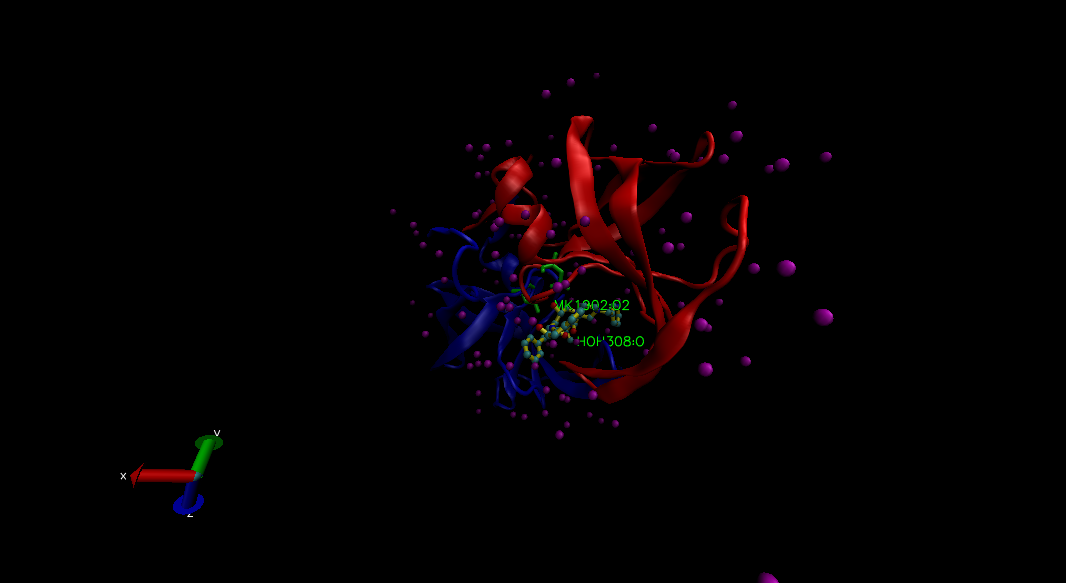
\includegraphics{rendered_1hsg_image.png}

\begin{quote}
\textbf{Discussion Topic:} Can you think of a way in which indinavir, or
even larger ligands and substrates, could enter the binding site?
{[}OPTIONAL{]}
\end{quote}

\hypertarget{sequence-viewer-extension-optional}{%
\subsection{Sequence Viewer Extension
{[}OPTIONAL{]}}\label{sequence-viewer-extension-optional}}

\begin{quote}
\textbf{Q6:} As you have hopefully observed HIV protease is a homodimer
(i.e.~it is composed of two identical chains). With the aid of the
graphic display and the sequence viewer extension can you identify
secondary structure elements that are likely to only form in the dimer
rather than the monomer? {[}OPTIONAL{]}
\end{quote}

\hypertarget{introduction-to-bio3d-in-r}{%
\section{3. Introduction to Bio3D in
R}\label{introduction-to-bio3d-in-r}}

\hypertarget{reading-pdb-file-data-into-r}{%
\subsection{Reading PDB file data into
R}\label{reading-pdb-file-data-into-r}}

\begin{Shaded}
\begin{Highlighting}[]
\FunctionTok{library}\NormalTok{(bio3d)}

\NormalTok{pdb }\OtherTok{\textless{}{-}} \FunctionTok{read.pdb}\NormalTok{(}\StringTok{"1hel"}\NormalTok{)}
\end{Highlighting}
\end{Shaded}

\begin{verbatim}
##   Note: Accessing on-line PDB file
\end{verbatim}

\begin{Shaded}
\begin{Highlighting}[]
\NormalTok{pdb}
\end{Highlighting}
\end{Shaded}

\begin{verbatim}
## 
##  Call:  read.pdb(file = "1hel")
## 
##    Total Models#: 1
##      Total Atoms#: 1186,  XYZs#: 3558  Chains#: 1  (values: A)
## 
##      Protein Atoms#: 1001  (residues/Calpha atoms#: 129)
##      Nucleic acid Atoms#: 0  (residues/phosphate atoms#: 0)
## 
##      Non-protein/nucleic Atoms#: 185  (residues: 185)
##      Non-protein/nucleic resid values: [ HOH (185) ]
## 
##    Protein sequence:
##       KVFGRCELAAAMKRHGLDNYRGYSLGNWVCAAKFESNFNTQATNRNTDGSTDYGILQINS
##       RWWCNDGRTPGSRNLCNIPCSALLSSDITASVNCAKKIVSDGNGMNAWVAWRNRCKGTDV
##       QAWIRGCRL
## 
## + attr: atom, xyz, seqres, helix, sheet,
##         calpha, remark, call
\end{verbatim}

\begin{Shaded}
\begin{Highlighting}[]
\FunctionTok{head}\NormalTok{(pdb}\SpecialCharTok{$}\NormalTok{atom)}
\end{Highlighting}
\end{Shaded}

\begin{verbatim}
##   type eleno elety  alt resid chain resno insert      x      y      z o     b
## 1 ATOM     1     N <NA>   LYS     A     1   <NA>  3.294 10.164 10.266 1 11.18
## 2 ATOM     2    CA <NA>   LYS     A     1   <NA>  2.388 10.533  9.168 1  9.68
## 3 ATOM     3     C <NA>   LYS     A     1   <NA>  2.438 12.049  8.889 1 14.00
## 4 ATOM     4     O <NA>   LYS     A     1   <NA>  2.406 12.898  9.815 1 14.00
## 5 ATOM     5    CB <NA>   LYS     A     1   <NA>  0.949 10.101  9.559 1 13.29
## 6 ATOM     6    CG <NA>   LYS     A     1   <NA> -0.050 10.621  8.573 1 13.52
##   segid elesy charge
## 1  <NA>     N   <NA>
## 2  <NA>     C   <NA>
## 3  <NA>     C   <NA>
## 4  <NA>     O   <NA>
## 5  <NA>     C   <NA>
## 6  <NA>     C   <NA>
\end{verbatim}

\begin{quote}
\textbf{Q7:} How many amino acid residues are there in this pdb object?
\end{quote}

\hypertarget{amino-acid-residues}{%
\subsubsection{185 amino acid residues}\label{amino-acid-residues}}

\begin{quote}
\textbf{Q8:} Name one of the two non-protein residues?
\end{quote}

\hypertarget{water}{%
\subsubsection{Water}\label{water}}

\begin{quote}
\textbf{Q9:} How many protein chains are in this structure?
\end{quote}

\hypertarget{two-protein-chains}{%
\subsubsection{Two protein chains}\label{two-protein-chains}}

Let's do a quick bioinformatics prediction of protein dynamics
(flexibility). We'll use the Normal Mode Analysis (NMA) function, a
prediction of the conformational variability and intrinsic dynamics of
this protein.

\begin{Shaded}
\begin{Highlighting}[]
\NormalTok{pdb }\OtherTok{\textless{}{-}} \FunctionTok{read.pdb}\NormalTok{(}\StringTok{"1hel"}\NormalTok{)}
\end{Highlighting}
\end{Shaded}

\begin{verbatim}
##   Note: Accessing on-line PDB file
\end{verbatim}

\begin{verbatim}
## Warning in get.pdb(file, path = tempdir(), verbose = FALSE): C:
## \Users\colta\AppData\Local\Temp\RtmpuqPPrc/1hel.pdb exists. Skipping download
\end{verbatim}

\begin{Shaded}
\begin{Highlighting}[]
\NormalTok{modes }\OtherTok{\textless{}{-}} \FunctionTok{nma}\NormalTok{(pdb)}
\end{Highlighting}
\end{Shaded}

\begin{verbatim}
##  Building Hessian...     Done in 0.01 seconds.
##  Diagonalizing Hessian...    Done in 0.15 seconds.
\end{verbatim}

\begin{Shaded}
\begin{Highlighting}[]
\FunctionTok{plot}\NormalTok{(modes)}
\end{Highlighting}
\end{Shaded}

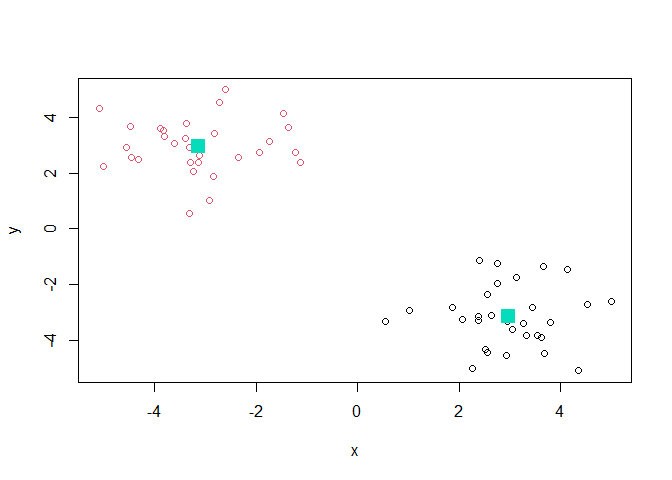
\includegraphics{lab11_files/figure-latex/unnamed-chunk-6-1.pdf}

Make a movie (trajectory) of this prediction for viewing in VMD using
`mktrj()'.

\begin{Shaded}
\begin{Highlighting}[]
\FunctionTok{mktrj}\NormalTok{(modes, }\AttributeTok{file =} \StringTok{"nma.pdb"}\NormalTok{)}
\CommentTok{\# Open as a \textquotesingle{}new molecule\textquotesingle{} in VMD then adjust graphic representation and press play.}
\CommentTok{\# In trajectory tab of the graphic representation change the \textquotesingle{}now\textquotesingle{} to \textquotesingle{}1:100\textquotesingle{} to render a still image.}
\end{Highlighting}
\end{Shaded}

Add the image from VMD

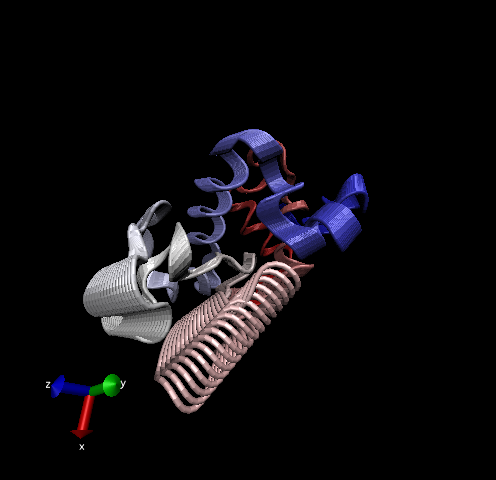
\includegraphics{nma.tga.png}

\hypertarget{comparative-structure-analysis-of-adenylate-kinase}{%
\section{4. Comparative structure analysis of Adenylate
Kinase}\label{comparative-structure-analysis-of-adenylate-kinase}}

\hypertarget{overview}{%
\subsection{Overview}\label{overview}}

Starting from only one Adk PDB identifier (PDB ID: 1AKE) we will search
the entire PDB for related structures using BLAST, fetch, align and
superpose the identified structures, perform PCA and finally calculate
the normal modes of each individual structure in order to probe for
potential differences in structural flexibility.

\begin{quote}
\textbf{Q10.} Which of the packages above is found only on BioConductor
and not CRAN?
\end{quote}

\hypertarget{msa}{%
\subsubsection{"msa'}\label{msa}}

\begin{quote}
\textbf{Q11.} Which of the above packages is not found on BioConductor
or CRAN?:
\end{quote}

\hypertarget{grantlabbio3d-view}{%
\subsubsection{``Grantlab/bio3d-view''}\label{grantlabbio3d-view}}

\begin{quote}
\textbf{Q12.} True or False? Functions from the devtools package can be
used to install packages from GitHub and BitBucket?
\end{quote}

\hypertarget{true}{%
\subsubsection{TRUE}\label{true}}

\hypertarget{search-and-retrieve-adk-structures}{%
\subsection{Search and retrieve ADK
structures}\label{search-and-retrieve-adk-structures}}

\begin{Shaded}
\begin{Highlighting}[]
\CommentTok{\# load previously run files to save time}
\FunctionTok{load}\NormalTok{(}\StringTok{"myresults.RData"}\NormalTok{)}
\end{Highlighting}
\end{Shaded}

\begin{Shaded}
\begin{Highlighting}[]
\CommentTok{\# Start by getting a sequence of interest}
\CommentTok{\# aa \textless{}{-} get.seq("1AKE\_A")}
\NormalTok{aa}
\end{Highlighting}
\end{Shaded}

\begin{verbatim}
##              1        .         .         .         .         .         60 
## pdb|1AKE|A   MRIILLGAPGAGKGTQAQFIMEKYGIPQISTGDMLRAAVKSGSELGKQAKDIMDAGKLVT
##              1        .         .         .         .         .         60 
## 
##             61        .         .         .         .         .         120 
## pdb|1AKE|A   DELVIALVKERIAQEDCRNGFLLDGFPRTIPQADAMKEAGINVDYVLEFDVPDELIVDRI
##             61        .         .         .         .         .         120 
## 
##            121        .         .         .         .         .         180 
## pdb|1AKE|A   VGRRVHAPSGRVYHVKFNPPKVEGKDDVTGEELTTRKDDQEETVRKRLVEYHQMTAPLIG
##            121        .         .         .         .         .         180 
## 
##            181        .         .         .   214 
## pdb|1AKE|A   YYSKEAEAGNTKYAKVDGTKPVAEVRADLEKILG
##            181        .         .         .   214 
## 
## Call:
##   read.fasta(file = outfile)
## 
## Class:
##   fasta
## 
## Alignment dimensions:
##   1 sequence rows; 214 position columns (214 non-gap, 0 gap) 
## 
## + attr: id, ali, call
\end{verbatim}

\begin{quote}
\textbf{Q13.} How many amino acids are in this sequence, i.e.~how long
is this sequence?
\end{quote}

\hypertarget{amino-acids}{%
\subsubsection{214 amino acids}\label{amino-acids}}

Search the PDB database (the main db for exp structures) for sequences
like my ``aa'' sequence.

\begin{Shaded}
\begin{Highlighting}[]
\CommentTok{\# blast \textless{}{-} blast.pdb(aa)}
\end{Highlighting}
\end{Shaded}

\begin{Shaded}
\begin{Highlighting}[]
\NormalTok{hits }\OtherTok{\textless{}{-}} \FunctionTok{plot}\NormalTok{(blast)}
\end{Highlighting}
\end{Shaded}

\begin{verbatim}
##   * Possible cutoff values:    197 -3 
##             Yielding Nhits:    16 100 
## 
##   * Chosen cutoff value of:    197 
##             Yielding Nhits:    16
\end{verbatim}

\includegraphics{lab11_files/figure-latex/unnamed-chunk-11-1.pdf}

Now I have my tops hits from the search of the PDB

\begin{Shaded}
\begin{Highlighting}[]
\CommentTok{\# Let\textquotesingle{}s look at the structure identifiers}
\NormalTok{hits}\SpecialCharTok{$}\NormalTok{pdb.id}
\end{Highlighting}
\end{Shaded}

\begin{verbatim}
##  [1] "1AKE_A" "4X8M_A" "6S36_A" "6RZE_A" "4X8H_A" "3HPR_A" "1E4V_A" "5EJE_A"
##  [9] "1E4Y_A" "3X2S_A" "6HAP_A" "6HAM_A" "4K46_A" "4NP6_A" "3GMT_A" "4PZL_A"
\end{verbatim}

Here we download all these similar structures in the PDB and store them
on our computer.

\begin{Shaded}
\begin{Highlighting}[]
\CommentTok{\# Download related PDB files}
\CommentTok{\# files \textless{}{-} get.pdb(hits$pdb.id, path = "pdbs", split = TRUE, gzip = TRUE)}
\end{Highlighting}
\end{Shaded}

\hypertarget{align-and-superpose-structures}{%
\subsection{Align and superpose
structures}\label{align-and-superpose-structures}}

We will use the function `pdbaln()' which requires a MUSCLE download.
Downloaded MUSCLE in the `Terminal' tab using: curl -o ``muscle.exe''
``\url{https://www.drive5.com/muscle/downloads3.8.31/muscle3.8.31_i86win32.exe}''

\begin{Shaded}
\begin{Highlighting}[]
\CommentTok{\# Align releated PDBs}
\NormalTok{pdbs }\OtherTok{\textless{}{-}} \FunctionTok{pdbaln}\NormalTok{(files, }\AttributeTok{fit =} \ConstantTok{TRUE}\NormalTok{)}
\end{Highlighting}
\end{Shaded}

\begin{verbatim}
## Reading PDB files:
## pdbs/split_chain/1AKE_A.pdb
## pdbs/split_chain/4X8M_A.pdb
## pdbs/split_chain/6S36_A.pdb
## pdbs/split_chain/6RZE_A.pdb
## pdbs/split_chain/4X8H_A.pdb
## pdbs/split_chain/3HPR_A.pdb
## pdbs/split_chain/1E4V_A.pdb
## pdbs/split_chain/5EJE_A.pdb
## pdbs/split_chain/1E4Y_A.pdb
## pdbs/split_chain/3X2S_A.pdb
## pdbs/split_chain/6HAP_A.pdb
## pdbs/split_chain/6HAM_A.pdb
## pdbs/split_chain/4K46_A.pdb
## pdbs/split_chain/4NP6_A.pdb
## pdbs/split_chain/3GMT_A.pdb
## pdbs/split_chain/4PZL_A.pdb
##    PDB has ALT records, taking A only, rm.alt=TRUE
## ..   PDB has ALT records, taking A only, rm.alt=TRUE
## .   PDB has ALT records, taking A only, rm.alt=TRUE
## ..   PDB has ALT records, taking A only, rm.alt=TRUE
## ..   PDB has ALT records, taking A only, rm.alt=TRUE
## ....   PDB has ALT records, taking A only, rm.alt=TRUE
## .   PDB has ALT records, taking A only, rm.alt=TRUE
## ....
## 
## Extracting sequences
## 
## pdb/seq: 1   name: pdbs/split_chain/1AKE_A.pdb 
##    PDB has ALT records, taking A only, rm.alt=TRUE
## pdb/seq: 2   name: pdbs/split_chain/4X8M_A.pdb 
## pdb/seq: 3   name: pdbs/split_chain/6S36_A.pdb 
##    PDB has ALT records, taking A only, rm.alt=TRUE
## pdb/seq: 4   name: pdbs/split_chain/6RZE_A.pdb 
##    PDB has ALT records, taking A only, rm.alt=TRUE
## pdb/seq: 5   name: pdbs/split_chain/4X8H_A.pdb 
## pdb/seq: 6   name: pdbs/split_chain/3HPR_A.pdb 
##    PDB has ALT records, taking A only, rm.alt=TRUE
## pdb/seq: 7   name: pdbs/split_chain/1E4V_A.pdb 
## pdb/seq: 8   name: pdbs/split_chain/5EJE_A.pdb 
##    PDB has ALT records, taking A only, rm.alt=TRUE
## pdb/seq: 9   name: pdbs/split_chain/1E4Y_A.pdb 
## pdb/seq: 10   name: pdbs/split_chain/3X2S_A.pdb 
## pdb/seq: 11   name: pdbs/split_chain/6HAP_A.pdb 
## pdb/seq: 12   name: pdbs/split_chain/6HAM_A.pdb 
##    PDB has ALT records, taking A only, rm.alt=TRUE
## pdb/seq: 13   name: pdbs/split_chain/4K46_A.pdb 
##    PDB has ALT records, taking A only, rm.alt=TRUE
## pdb/seq: 14   name: pdbs/split_chain/4NP6_A.pdb 
## pdb/seq: 15   name: pdbs/split_chain/3GMT_A.pdb 
## pdb/seq: 16   name: pdbs/split_chain/4PZL_A.pdb
\end{verbatim}

\begin{Shaded}
\begin{Highlighting}[]
\CommentTok{\# Vector containing PDB codes for figure axis}
\NormalTok{ids }\OtherTok{\textless{}{-}} \FunctionTok{basename.pdb}\NormalTok{(pdbs}\SpecialCharTok{$}\NormalTok{id)}

\CommentTok{\# Draw schematic alignment}
\FunctionTok{plot}\NormalTok{(pdbs, }\AttributeTok{labels=}\NormalTok{ids)}
\end{Highlighting}
\end{Shaded}

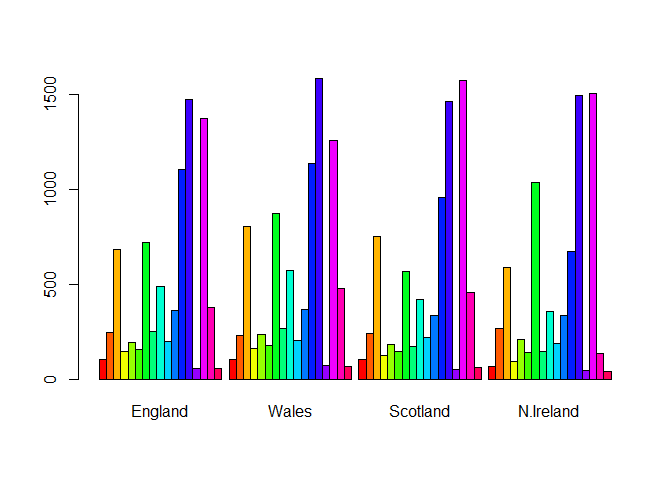
\includegraphics{lab11_files/figure-latex/unnamed-chunk-15-1.pdf}

Let's save our important results

\begin{Shaded}
\begin{Highlighting}[]
\FunctionTok{save}\NormalTok{(blast, hits, aa, files, }\AttributeTok{file =} \StringTok{"myresults.RData"}\NormalTok{)}
\end{Highlighting}
\end{Shaded}

\hypertarget{principle-component-analysis}{%
\subsection{Principle Component
Analysis}\label{principle-component-analysis}}

\begin{Shaded}
\begin{Highlighting}[]
\CommentTok{\# Perform PCA}
\NormalTok{pc.xray }\OtherTok{\textless{}{-}} \FunctionTok{pca}\NormalTok{(pdbs)}
\FunctionTok{plot}\NormalTok{(pc.xray)}
\end{Highlighting}
\end{Shaded}

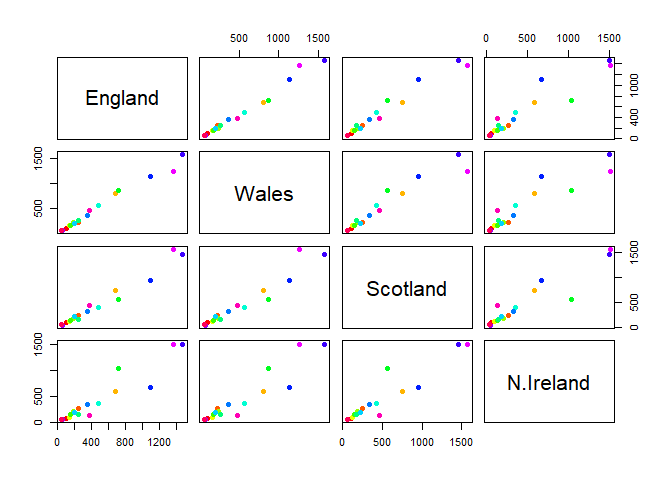
\includegraphics{lab11_files/figure-latex/unnamed-chunk-17-1.pdf}

\begin{Shaded}
\begin{Highlighting}[]
\CommentTok{\# Calculate RMSD}
\NormalTok{rd }\OtherTok{\textless{}{-}} \FunctionTok{rmsd}\NormalTok{(pdbs)}
\end{Highlighting}
\end{Shaded}

\begin{verbatim}
## Warning in rmsd(pdbs): No indices provided, using the 204 non NA positions
\end{verbatim}

\begin{Shaded}
\begin{Highlighting}[]
\CommentTok{\# Structure{-}based clustering}
\NormalTok{hc.rd }\OtherTok{\textless{}{-}} \FunctionTok{hclust}\NormalTok{(}\FunctionTok{dist}\NormalTok{(rd))}
\NormalTok{grps.rd }\OtherTok{\textless{}{-}} \FunctionTok{cutree}\NormalTok{(hc.rd, }\AttributeTok{k=}\DecValTok{3}\NormalTok{)}

\FunctionTok{plot}\NormalTok{(pc.xray, }\DecValTok{1}\SpecialCharTok{:}\DecValTok{2}\NormalTok{, }\AttributeTok{col=}\StringTok{"grey50"}\NormalTok{, }\AttributeTok{bg=}\NormalTok{grps.rd, }\AttributeTok{pch=}\DecValTok{21}\NormalTok{, }\AttributeTok{cex=}\DecValTok{1}\NormalTok{)}
\end{Highlighting}
\end{Shaded}

\includegraphics{lab11_files/figure-latex/unnamed-chunk-18-1.pdf}

\hypertarget{optional-further-visualization}{%
\section{5. Optional further
visualization}\label{optional-further-visualization}}

\begin{Shaded}
\begin{Highlighting}[]
\CommentTok{\# Visualize first principal component}
\NormalTok{pc1 }\OtherTok{\textless{}{-}} \FunctionTok{mktrj}\NormalTok{(pc.xray, }\AttributeTok{pc=}\DecValTok{1}\NormalTok{, }\AttributeTok{file=}\StringTok{"pc\_1.pdb"}\NormalTok{)}
\end{Highlighting}
\end{Shaded}

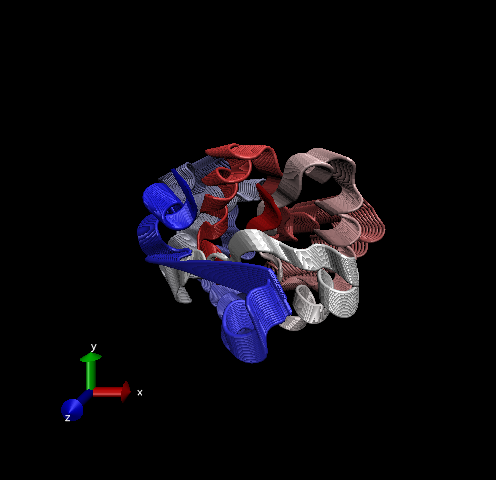
\includegraphics{1AKE_A image.png}

\begin{Shaded}
\begin{Highlighting}[]
\CommentTok{\#Plotting results with ggplot2}
\FunctionTok{library}\NormalTok{(ggplot2)}
\FunctionTok{library}\NormalTok{(ggrepel)}

\NormalTok{df }\OtherTok{\textless{}{-}} \FunctionTok{data.frame}\NormalTok{(}\AttributeTok{PC1=}\NormalTok{pc.xray}\SpecialCharTok{$}\NormalTok{z[,}\DecValTok{1}\NormalTok{], }
                 \AttributeTok{PC2=}\NormalTok{pc.xray}\SpecialCharTok{$}\NormalTok{z[,}\DecValTok{2}\NormalTok{], }
                 \AttributeTok{col=}\FunctionTok{as.factor}\NormalTok{(grps.rd),}
                 \AttributeTok{ids=}\NormalTok{ids)}

\NormalTok{p }\OtherTok{\textless{}{-}} \FunctionTok{ggplot}\NormalTok{(df) }\SpecialCharTok{+} 
  \FunctionTok{aes}\NormalTok{(PC1, PC2, }\AttributeTok{col=}\NormalTok{col, }\AttributeTok{label=}\NormalTok{ids) }\SpecialCharTok{+}
  \FunctionTok{geom\_point}\NormalTok{(}\AttributeTok{size=}\DecValTok{2}\NormalTok{) }\SpecialCharTok{+}
  \FunctionTok{geom\_text\_repel}\NormalTok{(}\AttributeTok{max.overlaps =} \DecValTok{20}\NormalTok{) }\SpecialCharTok{+}
  \FunctionTok{theme}\NormalTok{(}\AttributeTok{legend.position =} \StringTok{"none"}\NormalTok{)}
\NormalTok{p}
\end{Highlighting}
\end{Shaded}

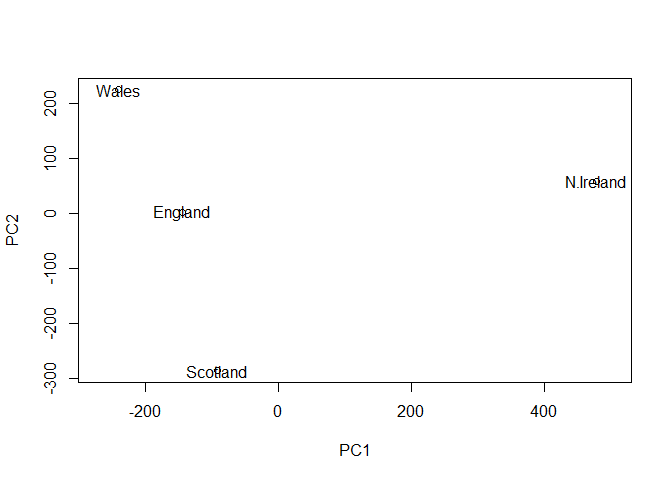
\includegraphics{lab11_files/figure-latex/unnamed-chunk-20-1.pdf}

\hypertarget{normal-mode-analysis}{%
\section{6. Normal mode analysis}\label{normal-mode-analysis}}

\begin{Shaded}
\begin{Highlighting}[]
\CommentTok{\# NMA of all structures}
\NormalTok{modes }\OtherTok{\textless{}{-}} \FunctionTok{nma}\NormalTok{(pdbs)}
\end{Highlighting}
\end{Shaded}

\begin{verbatim}
## 
## Details of Scheduled Calculation:
##   ... 16 input structures 
##   ... storing 606 eigenvectors for each structure 
##   ... dimension of x$U.subspace: ( 612x606x16 )
##   ... coordinate superposition prior to NM calculation 
##   ... aligned eigenvectors (gap containing positions removed)  
##   ... estimated memory usage of final 'eNMA' object: 45.4 Mb 
## 
##   |                                                                              |                                                                      |   0%  |                                                                              |====                                                                  |   6%  |                                                                              |=========                                                             |  12%  |                                                                              |=============                                                         |  19%  |                                                                              |==================                                                    |  25%  |                                                                              |======================                                                |  31%  |                                                                              |==========================                                            |  38%  |                                                                              |===============================                                       |  44%  |                                                                              |===================================                                   |  50%  |                                                                              |=======================================                               |  56%  |                                                                              |============================================                          |  62%  |                                                                              |================================================                      |  69%  |                                                                              |====================================================                  |  75%  |                                                                              |=========================================================             |  81%  |                                                                              |=============================================================         |  88%  |                                                                              |==================================================================    |  94%  |                                                                              |======================================================================| 100%
\end{verbatim}

\begin{Shaded}
\begin{Highlighting}[]
\FunctionTok{plot}\NormalTok{(modes, pdbs, }\AttributeTok{col=}\NormalTok{grps.rd)}
\end{Highlighting}
\end{Shaded}

\begin{verbatim}
## Extracting SSE from pdbs$sse attribute
\end{verbatim}

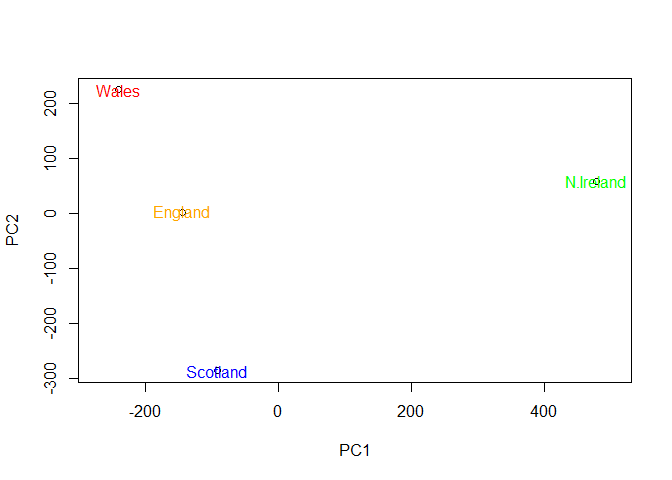
\includegraphics{lab11_files/figure-latex/unnamed-chunk-21-1.pdf}

\begin{quote}
\textbf{Q14.} What do you note about this plot? Are the black and
colored lines similar or different? Where do you think they differ most
and why?
\end{quote}

\end{document}
